\chapter{Installation and User Guide}

\section{Installation}

\subsection{Backend}

\subsubsection{Overview}

\textbf{FinSight} is an AI-powered financial analytics backend that provides news aggregation, vector-based retrieval, stock forecasting, recommendation, and RAG-based financial research assistance — all implemented within a modular \texttt{FastAPI} architecture.

This repository hosts the backend micro-services, which include:

\begin{itemize}
    \item \textbf{News Fetching \& Aggregation}
    \item \textbf{Stock Trend Forecasting} (ARIMA / Prophet / LSTM / LightGBM / Transformer / Seq2Seq)
    \item \textbf{RAG-based Financial Research Analyst}
    \item \textbf{Content-based \& Vector-based Stock Recommendation}
    \item \textbf{User Profiles, Watchlists, and Authentication}
    \item \textbf{MongoDB + Postgres (pgvector) Support}
\end{itemize}

\subsubsection{Project Structure}

\begin{lstlisting}[language={}, basicstyle=\ttfamily\small]
FinSight_BackEnd
├── app
│   ├── adapters
│   │   ├── db
│   │   │   ├── database_client.py
│   │   │   ├── news_repo.py
│   │   │   ├── pg_profile_repo.py
│   │   │   ├── rag_conversation_repo.py
│   │   │   └── user_repo.py
│   │   ├── embeddings
│   │   ├── fetchers
│   │   ├── llm
│   │   ├── rag
│   │   └── vector
│   ├── api
│   │   └── v1
│   │       ├── auth_router.py
│   │       ├── forecast_router.py
│   │       ├── news_router.py
│   │       ├── rag_router.py
│   │       ├── rec_router.py
│   │       ├── stocks_router.py
│   │       └── user_router.py
│   ├── forecasters
│   │   ├── arima_forecaster.py
│   │   ├── prophet_forecaster.py
│   │   ├── lstm_forecaster.py
│   │   ├── transformer_forecaster.py
│   │   └── stacked_forecaster.py
│   ├── services
│   │   ├── news_service.py
│   │   ├── forecast_service.py
│   │   ├── rag_service.py
│   │   ├── rec_service.py
│   │   └── user_service.py
│   └── main.py
├── docker-compose.yml
├── environment.yml
├── finsight_keypair.pem
├── pyproject.toml
├── README.md
└── requirements.txt
\end{lstlisting}

All dependencies are fully managed through \textbf{\texttt{pyproject.toml}}.

\subsubsection{Prerequisites}

\begin{table}[H]
\centering
\caption{System Prerequisites}
\begin{tabular}{|l|l|}
\hline
\textbf{Tool} & \textbf{Requirement} \\
\hline
Python & 3.10+ \\
Docker & Required for Knowledge Base (MongoDB + Postgres) \\
uv / pip & For dependency installation \\
Ragflow & For RAG deployment \\
Ollama & For local LLM provider \\
\hline
\end{tabular}
\end{table}

Installation of \texttt{uv}
\begin{lstlisting}[language=bash]
curl -LsSf https://astral.sh/uv/install.sh | sh
\end{lstlisting}

Database Access (via EC2 Server)

The EC2 server hosts both MongoDB and PostgreSQL databases:

\begin{itemize}
    \item \textbf{MongoDB:} Stores news and optionally vector embeddings.
    \item \textbf{PostgreSQL + pgvector:} Stores user profiles, embeddings, and recommendations.
\end{itemize}

To connect, simply place \texttt{finsight\_keypair.pem} in the project root.  
The program will automatically establish the SSH tunnel and access the databases.

\subsubsection{Optional: RAG Component Deployment}

Due to limited memory on the EC2 server, the RAG module is deployed locally.  
This step is optional and does not affect other backend functionalities.

\begin{enumerate}
    \item \textbf{Deploy Ragflow locally:} Follow the official guide at \texttt{https://ragflow.io/docs/dev/build\_docker\_image}.
    \item \textbf{Run local LLM via Ollama:}
    \begin{lstlisting}[language=bash]
    ollama run deepseek-r1:8b
    \end{lstlisting}
    \item \textbf{Replace your Ragflow key:}  
    Add it to the \texttt{.env} file as:
    \begin{lstlisting}
    RAGFLOW_API_KEY=<your-key>
    \end{lstlisting}
\end{enumerate}

\subsubsection{Installation}

\begin{lstlisting}[language=bash]
git clone https://github.com/jiajun-lab/FinSight_BackEnd.git FinSight_BackEnd
cd FinSight_BackEnd

# Create virtual environment
uv venv
source .venv/bin/activate

# Install dependencies
uv pip install -e .
# (or pip install -e .)
\end{lstlisting}

\textbf{Note:} Prophet will compile CmdStan on first run, which may take several minutes.

\subsubsection{Running the Backend}

Before starting, configure your \texttt{.env} file accordingly.

\begin{lstlisting}[language=bash]
uvicorn app.main:app --reload --port 8000
\end{lstlisting}

API documentation is available at:

\begin{lstlisting}
http://localhost:8000/docs
\end{lstlisting}

The backend service runs on \texttt{http://localhost:8000}, and the frontend retrieves all data from this endpoint.

---

\subsection{Frontend}
\subsubsection{Installation}

\begin{lstlisting}[language=bash]
# 1) Clone this repository
git clone https://github.com/jiajun-lab/FinSight_Frontend.git FinSight_FrontEnd
cd FinSight_FrontEnd

# 2) In this folder:
pnpm i

# 3) set backend endpoint (optional; default already localhost):
echo 'VITE_BACKEND_BASE_URL=http://127.0.0.1:8000' > .env

# 4) run
pnpm dev

# 5) quick restart
rm -rf node_modules pnpm-lock.yaml package-lock.json # optional clean reboot
pnpm i 
pnpm dev 
\end{lstlisting}



\section{News Browsing}

\subsection{Overview}

The FinSight News Browsing Module allows users to explore personalized financial news in an intuitive and interactive interface.  
The system learns from your actions --- such as reading, liking, and bookmarking --- to continuously refine future recommendations.  
This guide explains how to navigate, interact, and get the best experience from the news platform.

\subsection{Getting Started}

\begin{enumerate}
  \item Open the FinSight web application in your browser.
  \item Log in with your registered account.  
  \item Click on the \textbf{“News”} tab in the top navigation bar to enter the news recommendation page.
\end{enumerate}

Once you enter, the system automatically loads your personalized news feed, showing 9 recommended articles in a clean \(3\times3\) grid layout.

\subsection{Browsing the News Feed}

\begin{itemize}
  \item Each news card displays the \textbf{title}, \textbf{source}, \textbf{publication time}, and \textbf{related stock or sector}.
  \item Click the article title to open the full story in a new browser tab.
  \item Use the \textbf{Next} and \textbf{Previous} buttons at the bottom to move between pages.
  \item The system automatically caches previous pages, so navigation is fast and seamless.
  \item When you reach the last page and click \textbf{Next}, new articles will be fetched and displayed automatically.
\end{itemize}

\subsection{Interacting with Articles}

You can directly interact with each article to help the system learn your preferences:

\begin{itemize}
  \item \textbf{Like} (\(\heartsuit\)) — Press this button if you find an article relevant or interesting.  
        Future recommendations will prioritize similar topics or sectors.
  \item \textbf{Bookmark} (\(\star\)) — Use this to save an article for later reading.  
        It also signals a stronger preference to the system.
  \item \textbf{Read} — Simply clicking and reading an article contributes to your profile based on reading duration.
\end{itemize}

All actions update your profile automatically in the background --- there is no need to refresh the page.

\subsection{Getting Personalized Recommendations}

The news feed automatically adapts based on your reading and interaction history:
\begin{itemize}
  \item The more you interact, the more accurate your recommendations become.
  \item You will start seeing more articles from sectors and companies that match your interests.
  \item Older or irrelevant content will gradually fade out as new interests emerge.
\end{itemize}

You can always reset your browsing session by reloading the page --- the system will load a fresh selection of recommended articles.

\subsection{Tips for Best Experience}

\begin{itemize}
  \item Interact regularly (like or bookmark) to personalize your feed faster.
  \item Use \textbf{Next} to load new articles when you reach the end of your feed.
  \item The system automatically avoids showing repeated or recently viewed items.
  \item All updates happen instantly without page reloads.
\end{itemize}


\section{Stock Recommendation}

The Stock Recommendation System helps investors discover suitable investment opportunities through intelligent algorithms and comprehensive stock analysis tools. This manual explains how to use the six main features of the system.

\subsection{Browsing All Stocks}
To explore the complete stock universe:

\begin{enumerate}
    \item Click the \textbf{"All Stocks"} tab in the main navigation.
    \item Use the search bar at the top to find stocks by symbol or company name.
    \item Scroll through the grid layout to view all available stocks.
    \item Each stock card displays:
    \begin{itemize}
        \item Stock symbol and company name
        \item Sector with color coding
        \item Basic financial metrics when available
    \end{itemize}
    \item Click the pagination controls at the bottom to navigate through multiple pages.
    \item Hover over any stock card to trigger pre-loading of detailed information.
\end{enumerate}

\subsection{Getting Basic Recommendations}
To receive personalized stock recommendations, as shown in Fig \ref{fig:basic_recommend}:

\begin{enumerate}
    \item Ensure you are logged in to your account
    \item Click the \textbf{"Recommended"} tab
    \item The system automatically displays stocks matching your investment profile
    \item Adjust recommendation settings:
    \begin{itemize}
        \item Use the \textbf{"Top K"} input to change the number of recommendations (1-20)
        \item Use the \textbf{"Diversity"} dropdown to control sector variety
    \end{itemize}
    \item Click the \textbf{"Refresh"} button to update recommendations
    \item Each recommendation shows a similarity score indicating how well it matches your profile
\end{enumerate}

\begin{figure}[H]
    \centering
    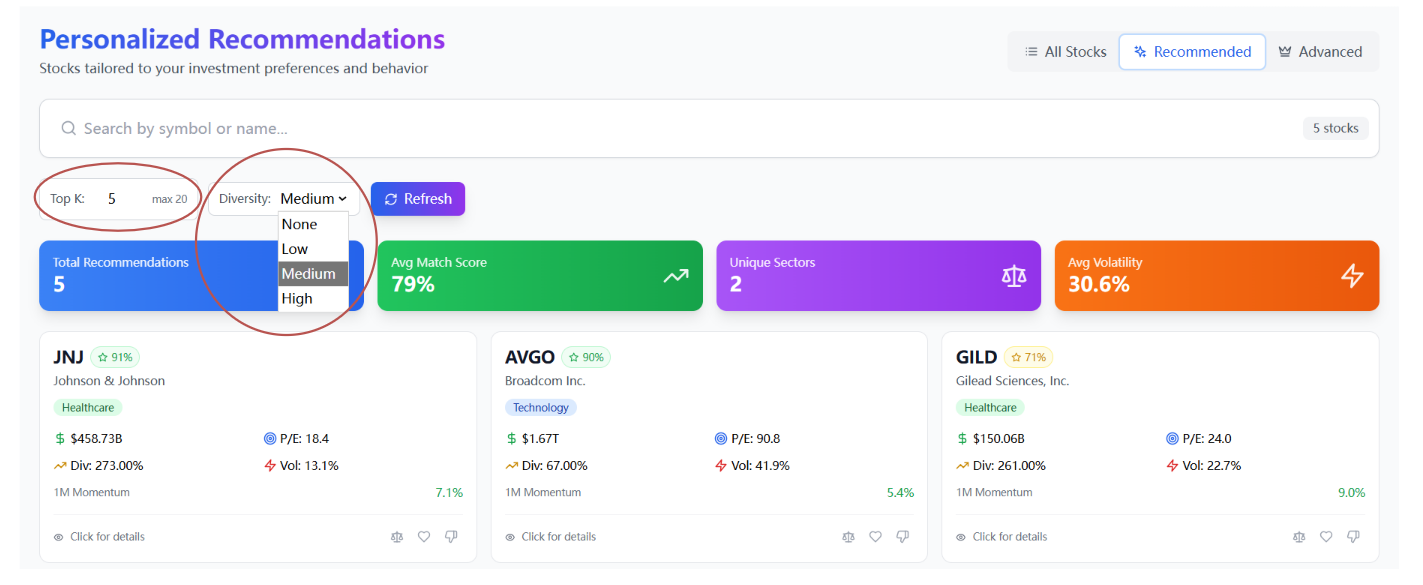
\includegraphics[width=1\linewidth]{images/stock_recommend/user_guide/basic_recommend.png}
    \caption{Basic Recommendation}
    \label{fig:basic_recommend}
\end{figure}


\subsection{Using Advanced Recommendations}
For multi-objective optimized recommendations, as Shown in Fig \ref{fig:advanced_recommend}:

\begin{enumerate}
    \item Click the \textbf{"Advanced"} tab
    \item Select your risk profile:
    \begin{itemize}
        \item \textbf{Conservative}: Lower risk, stable returns
        \item \textbf{Balanced}: Moderate risk and return balance
        \item \textbf{Aggressive}: Higher risk, potential for higher returns
    \end{itemize}
    \item View the detailed score breakdown for each recommendation:
    \begin{itemize}
        \item Final composite score
        \item Preference matching score
        \item Risk-adjusted return score
        \item Diversification benefit score
        \item Market timing score
    \end{itemize}
    \item Read the explanation for why each stock is recommended
    \item Adjust the number of recommendations using the \textbf{"Top K"} setting
\end{enumerate}

\begin{figure}[H]
    \centering
    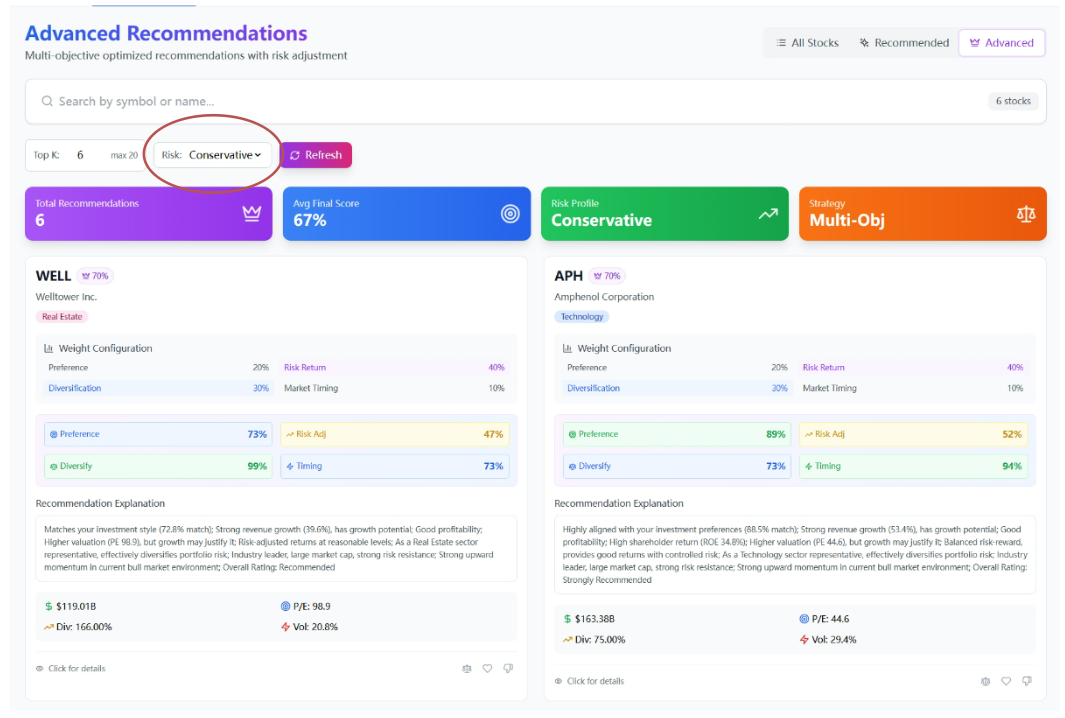
\includegraphics[width=1\linewidth]{images/stock_recommend/user_guide/advanced_recommend.png}
    \caption{Advanced Recommendation}
    \label{fig:advanced_recommend}
\end{figure}


\subsection{Comparing Stocks}
To compare multiple stocks side-by-side, as shown in Fig \ref{fig:stock_comparison}:

\begin{enumerate}
    \item Click the scale icon on any stock card to add it to comparison
    \item You can add up to 3 stocks for comparison
    \item View the comparison panel that appears at the top of the screen
    \item Click \textbf{"Analyze Comparison"} when you have 2 or more stocks selected
    \item In the comparison modal, you can:
    \begin{itemize}
        \item View side-by-side metrics in a comparison table
        \item Analyze valuation differences through bar charts
        \item Compare risk levels through volatility visualizations
        \item Review growth metric comparisons
        \item Read the summary analysis highlighting key differences
    \end{itemize}
    \item Remove stocks from comparison by clicking the 'x' button
\end{enumerate}
\begin{figure}[H]
    \centering
    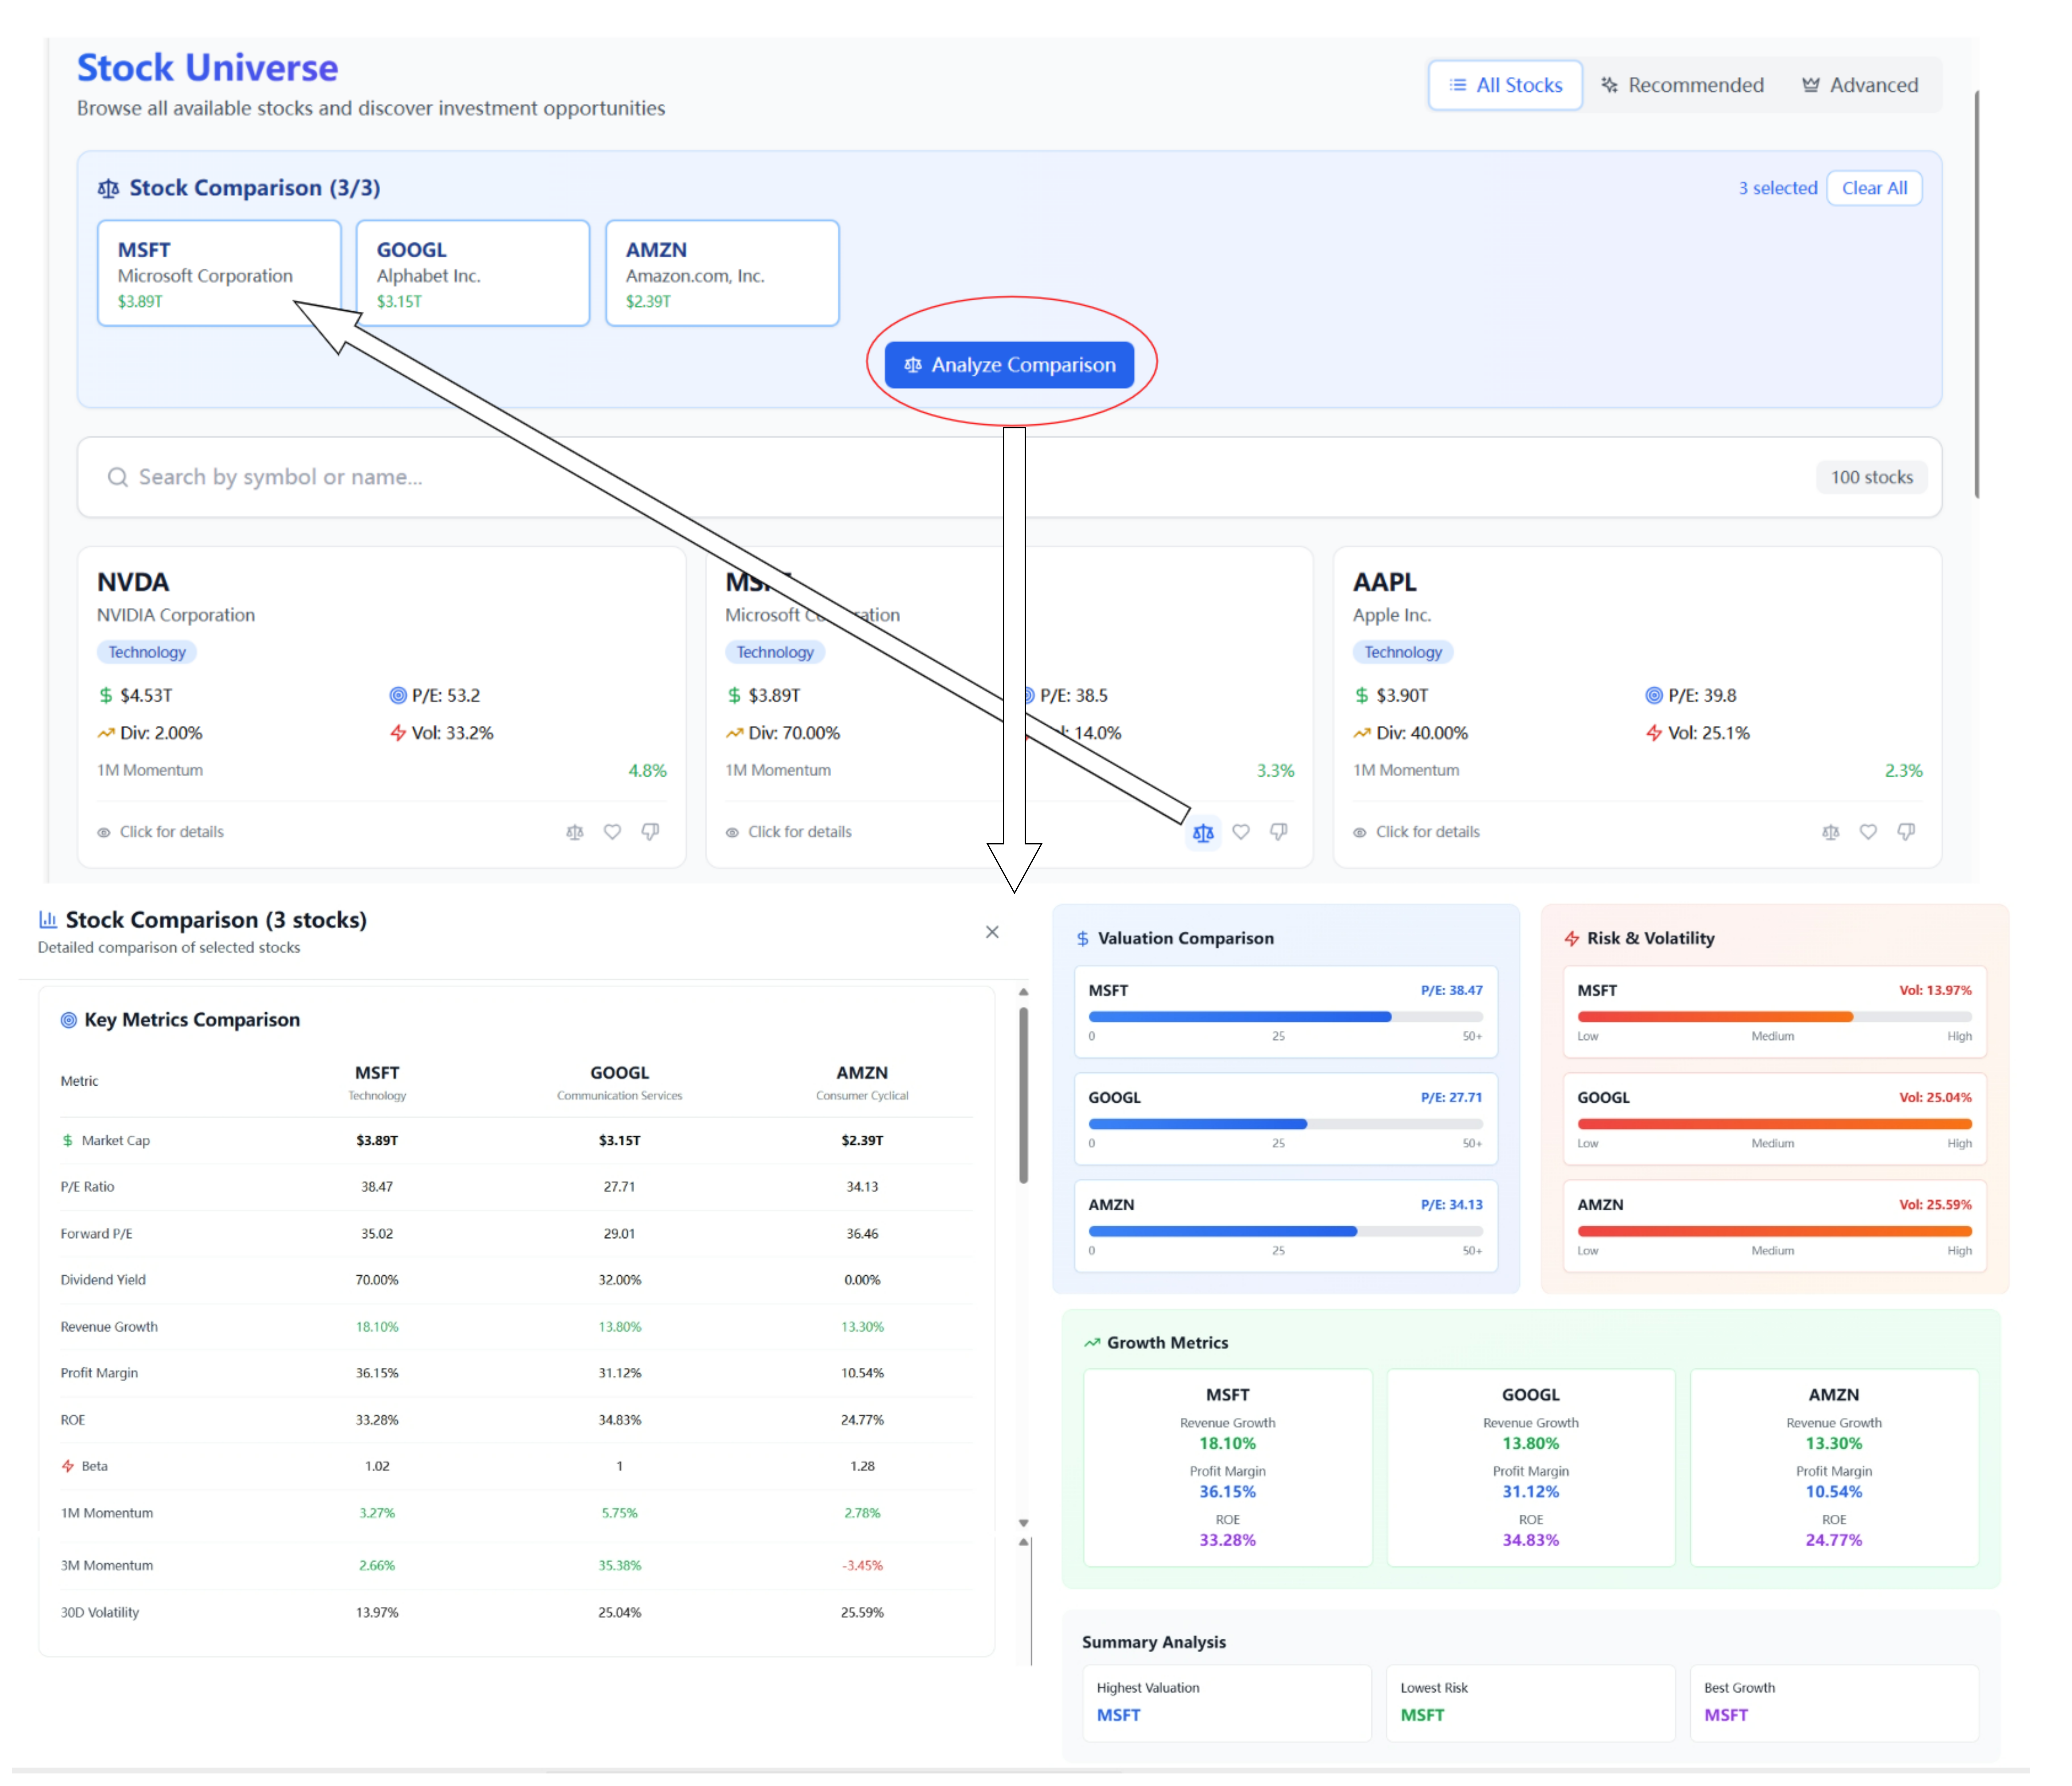
\includegraphics[width=1\linewidth]{images/stock_recommend/user_guide/compare.png}
    \caption{Stock Comparison}
    \label{fig:stock_comparison}
\end{figure}


\subsection{Viewing Stock Details}
To access comprehensive stock information, as shown in Fig \ref{fig:stock_detail}:

\begin{enumerate}
    \item Click on any stock card (except the action buttons)
    \item The stock detail modal will open with comprehensive information
    \item Navigate through different sections:
    \begin{itemize}
        \item \textbf{Price Charts}: Switch between time ranges (1M, 3M, 6M, 1Y) and price types (Close, Open, High, Low)
        \item \textbf{Valuation Metrics}: View P/E ratios, market cap, and other valuation data
        \item \textbf{Financial Ratios}: Analyze profitability, growth, and efficiency metrics
        \item \textbf{Dividend Information}: Review yield and payout ratios
        \item \textbf{Performance Metrics}: Check momentum and volatility data
        \item \textbf{Business Summary}: Read the company description
    \end{itemize}
\end{enumerate}

\begin{figure}[H]
    \centering
    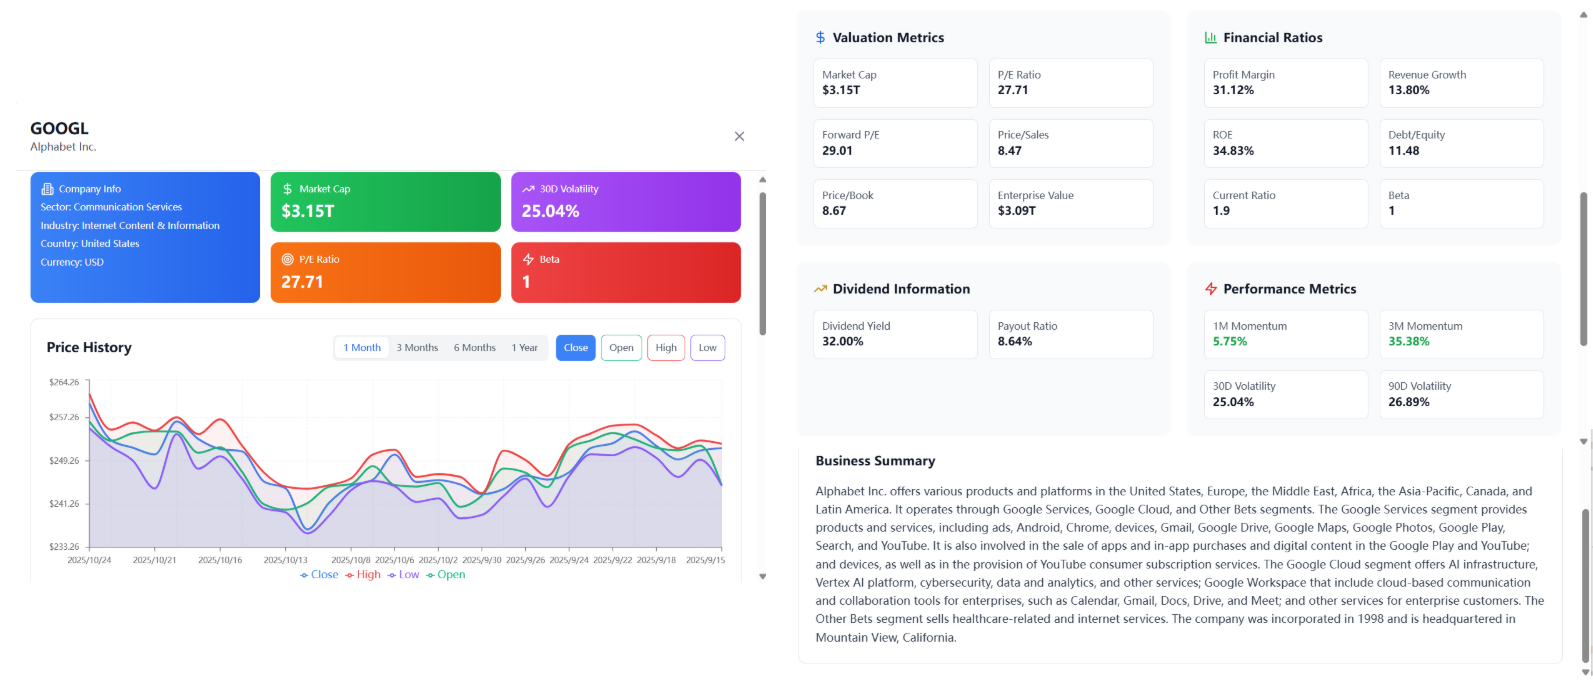
\includegraphics[width=1\linewidth]{images/stock_recommend/user_guide/stock_detail.png}
    \caption{Stock Detail}
    \label{fig:stock_detail}
\end{figure}

\subsection{Improving Recommendations Through Behavior}
The system learns from your interactions to provide better recommendations, as shown in Fig \ref{fig:like_dislike}:

\begin{enumerate}
    \item \textbf{Liking Stocks}: Click the heart icon ($\pmb{\heartsuit}$) on stocks you're interested in
    \begin{itemize}
        \item This tells the system you prefer similar stocks
        \item The heart will turn green and show a count
    \end{itemize}
    \item \textbf{Disliking Stocks}: Click the thumbs down icon on stocks you want to avoid
    \begin{itemize}
        \item This helps the system understand what to avoid recommending
        \item The icon will turn red and show a count
    \end{itemize}
    \item \textbf{Viewing Details}: Simply clicking on stocks to view details also influences your profile
    \item \textbf{Automatic Updates}: The system automatically:
    \begin{itemize}
        \item Updates your investment profile based on interactions
        \item Adjusts future recommendations in real-time
        \item Learns your sector preferences and investment style
    \end{itemize}
    \item To see the impact of your interactions, refresh the recommendations after several interactions
\end{enumerate}

\begin{figure}[H]
    \centering
    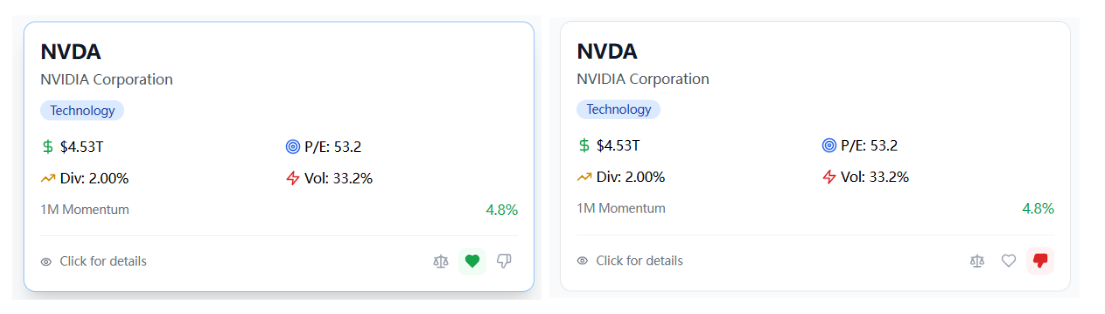
\includegraphics[width=1\linewidth]{images/stock_recommend/user_guide/like_dislike.png}
    \caption{User Behavior (like, dislike}
    \label{fig:like_dislike}
\end{figure}






\section{Stock Prediction}

\subsection{Overview}

The FinSight Stock Forecast Module provides users with intelligent, real-time stock trend predictions powered by multiple time-series and machine learning models.  
It visualizes both recent historical prices and short-term future forecasts, allowing users to intuitively interpret model predictions, confidence levels, and expected changes.  
This guide explains how to access, interact with, and interpret the stock forecasting interface.

\begin{figure}[H]
    \centering
    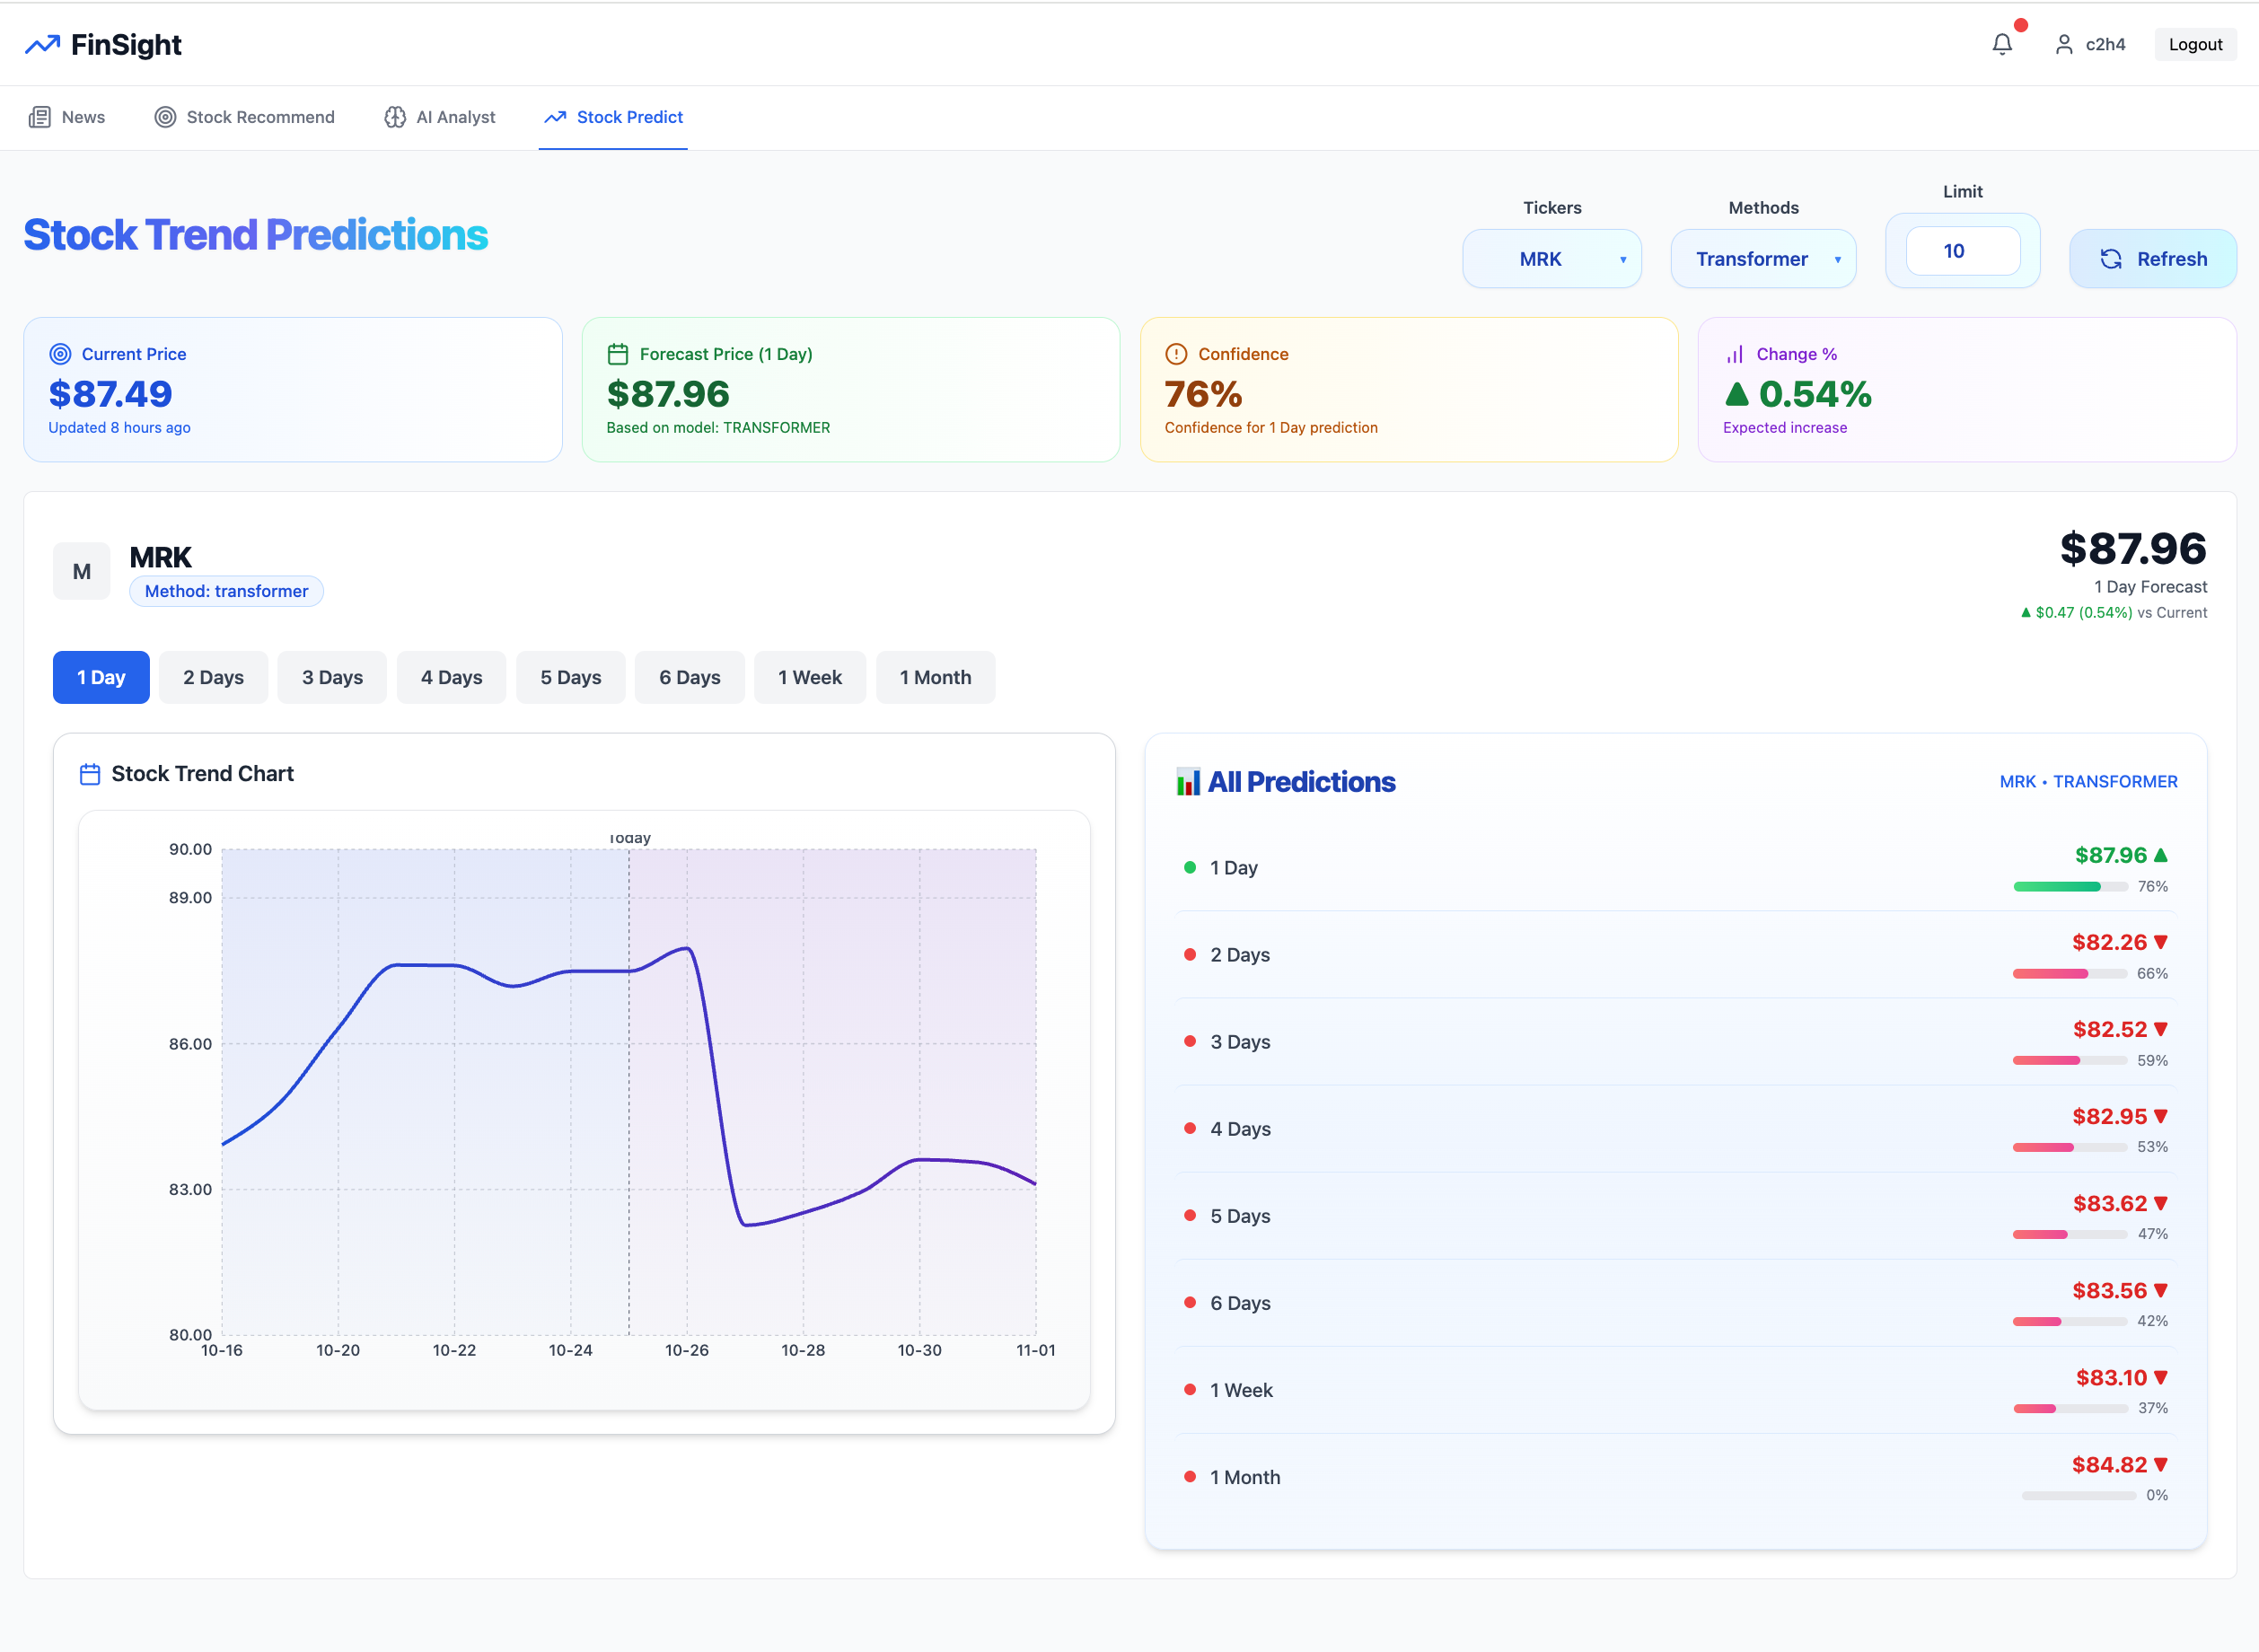
\includegraphics[width=1\linewidth]{images/prediction/overview.png}
    \caption{Stock Prediction User Interface}

\end{figure}

\subsection{Interface Overview}

\begin{enumerate}
  \item Open the FinSight web application in your browser.
  \item Log in using your registered account credentials.
  \item Navigate to the \textbf{“Stock Predict”} tab from the top navigation bar.
  \item Select a stock ticker (e.g., AAPL, TSLA, MRK) and a forecasting model (ARIMA, Prophet, LSTM, Transformer) from the dropdown menus.
  \item Click \textbf{Refresh} to load the most recent predictions and market data.
\end{enumerate}

Once loaded, the system displays the current price, forecasted price, model confidence, and expected percentage change in a clean and responsive dashboard.

\subsection{Understanding the Forecast Dashboard}

The main dashboard is divided into three functional regions for clarity and analytical insight:

\begin{itemize}
  \item \textbf{Top Summary Cards:}
    \begin{itemize}
      \item \textbf{Current Price:} Shows the latest closing price retrieved from the market data feed.
      \item \textbf{Forecast Price:} Displays the model’s predicted price for the selected horizon (e.g., 1 Day, 1 Week).
      \item \textbf{Confidence:} Indicates the model’s reliability, derived from validation metrics such as RMSE or variance.
      \item \textbf{Change} Shows the expected price movement relative to the current price, color-coded in green (positive) or red (negative).
    \end{itemize}
  \item \textbf{Trend Chart:}
    \begin{itemize}
      \item Visualizes both recent actual prices (solid blue line) and predicted prices (purple dashed line).
      \item A vertical line marks “today,” separating historical and forecasted data.
      \item Shaded areas represent confidence intervals for visualizing prediction uncertainty.
      \item Horizon buttons (1 Day, 3 Days, 1 Week, 1 Month) dynamically update the chart without reloading the page.
    \end{itemize}
  \item \textbf{Prediction Summary Panel:}
    \begin{itemize}
      \item Lists all horizon forecasts with predicted values, confidence scores, and trend arrows.
      \item Allows quick comparison between short-term and medium-term predictions.
      \item Color-coded bars visualize model confidence for each horizon.
    \end{itemize}
\end{itemize}

\subsection{Interacting with Forecasts}

You can explore predictions interactively:
\begin{itemize}
  \item Change the \textbf{ticker symbol} to analyze a different stock instantly.
  \item Switch between \textbf{models} (e.g., LSTM vs. Transformer) to compare forecast behavior.
  \item Adjust the \textbf{limit} or time horizon to view more or fewer prediction intervals.
  \item Hover over any data point in the chart to view exact date and price details.
\end{itemize}

All interactions automatically trigger backend API calls, and updated results appear within seconds.

\subsection{Interpreting Forecast Results}

\begin{itemize}
  \item A \textbf{higher confidence score} (close to 100\%) indicates a more stable forecast, while lower scores reflect market volatility or data uncertainty.
  \item Positive \textbf{Change \%} suggests an expected upward trend; negative values suggest possible price declines.
  \item Comparing multiple models provides insight into how traditional and deep learning approaches interpret market patterns differently.
  \item The chart’s shaded area width visually represents prediction risk—the wider the band, the greater the uncertainty.
\end{itemize}

\subsection{Tips for Best Experience}

\begin{itemize}
  \item Refresh periodically to fetch the most recent forecast data.
  \item Compare different models to assess prediction consistency.
  \item Use shorter horizons (1\–3 days) for near-term signals and longer ones for trend analysis.
  \item Interpret low-confidence predictions cautiously; they indicate volatile or sparse underlying data.
  \item Combine forecast insights with other FinSight modules for more informed investment decisions.
\end{itemize}




\section{AI Analyst}

The \textbf{AI Financial Analyst} module serves as an intelligent assistant powered by a Retrieval-Augmented Generation (RAG) framework. 
It enables users to ask analytical questions about stocks, sectors, earnings, and market trends, and receive context-aware, knowledge-grounded answers.
\begin{figure}[H]
    \centering
    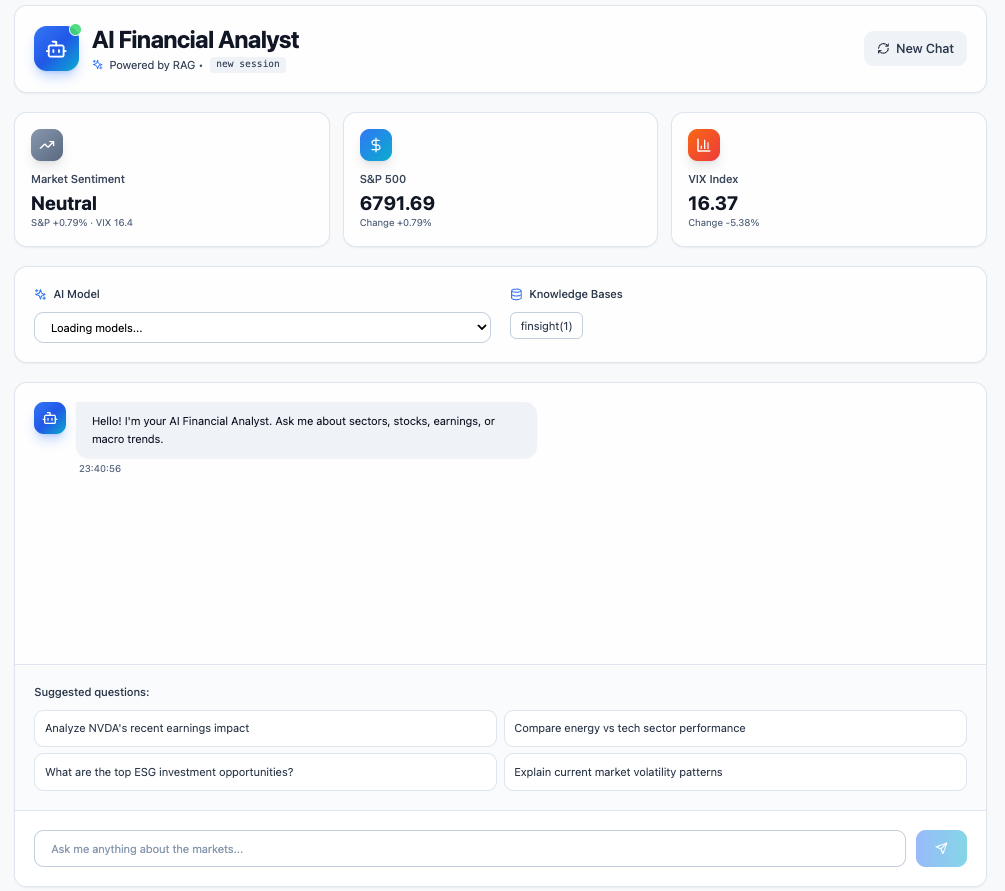
\includegraphics[width=1\linewidth]{images/AI_Analyst_interface.png}
    \caption{AI Analyst User Interface}
    \label{fig:placeholder}
\end{figure}
\subsection{Interface Overview}

\begin{itemize}
    \item \textbf{Market Indicators} \\
    The dashboard displays key real-time market metrics:
    \begin{itemize}
        \item \textbf{Market Sentiment:} General market mood derived from aggregated financial data.
        \item \textbf{S\&P 500 Index:} Current value and daily percentage change of the U.S. benchmark index.
        \item \textbf{VIX Index:} Market volatility indicator reflecting overall risk and uncertainty levels.
    \end{itemize}

    \item \textbf{AI Model Selection} \\
    Users can choose among available AI models (e.g., deepSeek-r1:8b) to power the assistant’s reasoning and response generation.

    \item \textbf{Knowledge Base Selection} \\
    The system allows users to select from available financial knowledge bases (e.g., \textit{finsight(1)}). 
    The selected dataset determines the retrieval source used to ground responses with relevant and accurate financial context.
\end{itemize}

\subsection{Functionality}

The AI Analyst supports natural-language financial Q\&A, allowing users to:
\begin{itemize}
    \item Ask about market movements, company performance, or sector comparisons.
    \item Obtain summarized insights, reasoning explanations, and evidence-based references.
    \item Conduct context-aware, multi-turn analytical conversations supported by the selected model and knowledge base.
\end{itemize}
